\section{The ATLAS experiment at the Large Hadron Collider}\label{sec:atlas}
Exploring the nature of the Higgs particle requires collision energies on the \qty[]{}{TeV} scale. The \ac{lhc} is currently the most powerful particle accelerator making it the best available facility for studying the Higgs particle. The main reference for this section is \citep{aad2008atlas}.

\subsection{The Large Hadron Collider}
The \ac{lhc} is a circular proton proton collider with \qty[]{27}{km} circumference with a center-of-mass energy of $\sqrt{s}=\qty[]{13}{TeV}$. The two anticyclic proton beams are actually bunches containing $10^{11}$ protons that are brought to collisions at several points of the ring for the experiments performed at the \ac{lhc}. A measure of how tightly particles are packed in these bunches is the instantaneous luminosity and is characteristic to the collider
\begin{equation}
    L=\frac{1}{\sigma}\frac{\dint{N}}{\dint{t}}.
\end{equation}
It can be read as particle interactions per unit time and area. The area understood as the interaction cross-section of a particular process. The total recorded number of collision events is then with the integrated luminosity 
\begin{equation}
    N=\sigma\cdot\int L dt=\sigma\cdot L_\mathrm{int}.
\end{equation}
For the full run 2 dataset used in this thesis the integrated luminosity for events good for physics analysis is \qty[]{140.1}{fb^{-1}}\citep{DAPR-2021-01}. When bunches are collided not only one but rather several proton-proton interactions are measured. Methods to disentangle the different interactions in the detector improved over time so the mean number of interactions also called pile up increased during the data taking period as can be seen in figure \ref{fig:pileup}.
\begin{figure}
    \centering
    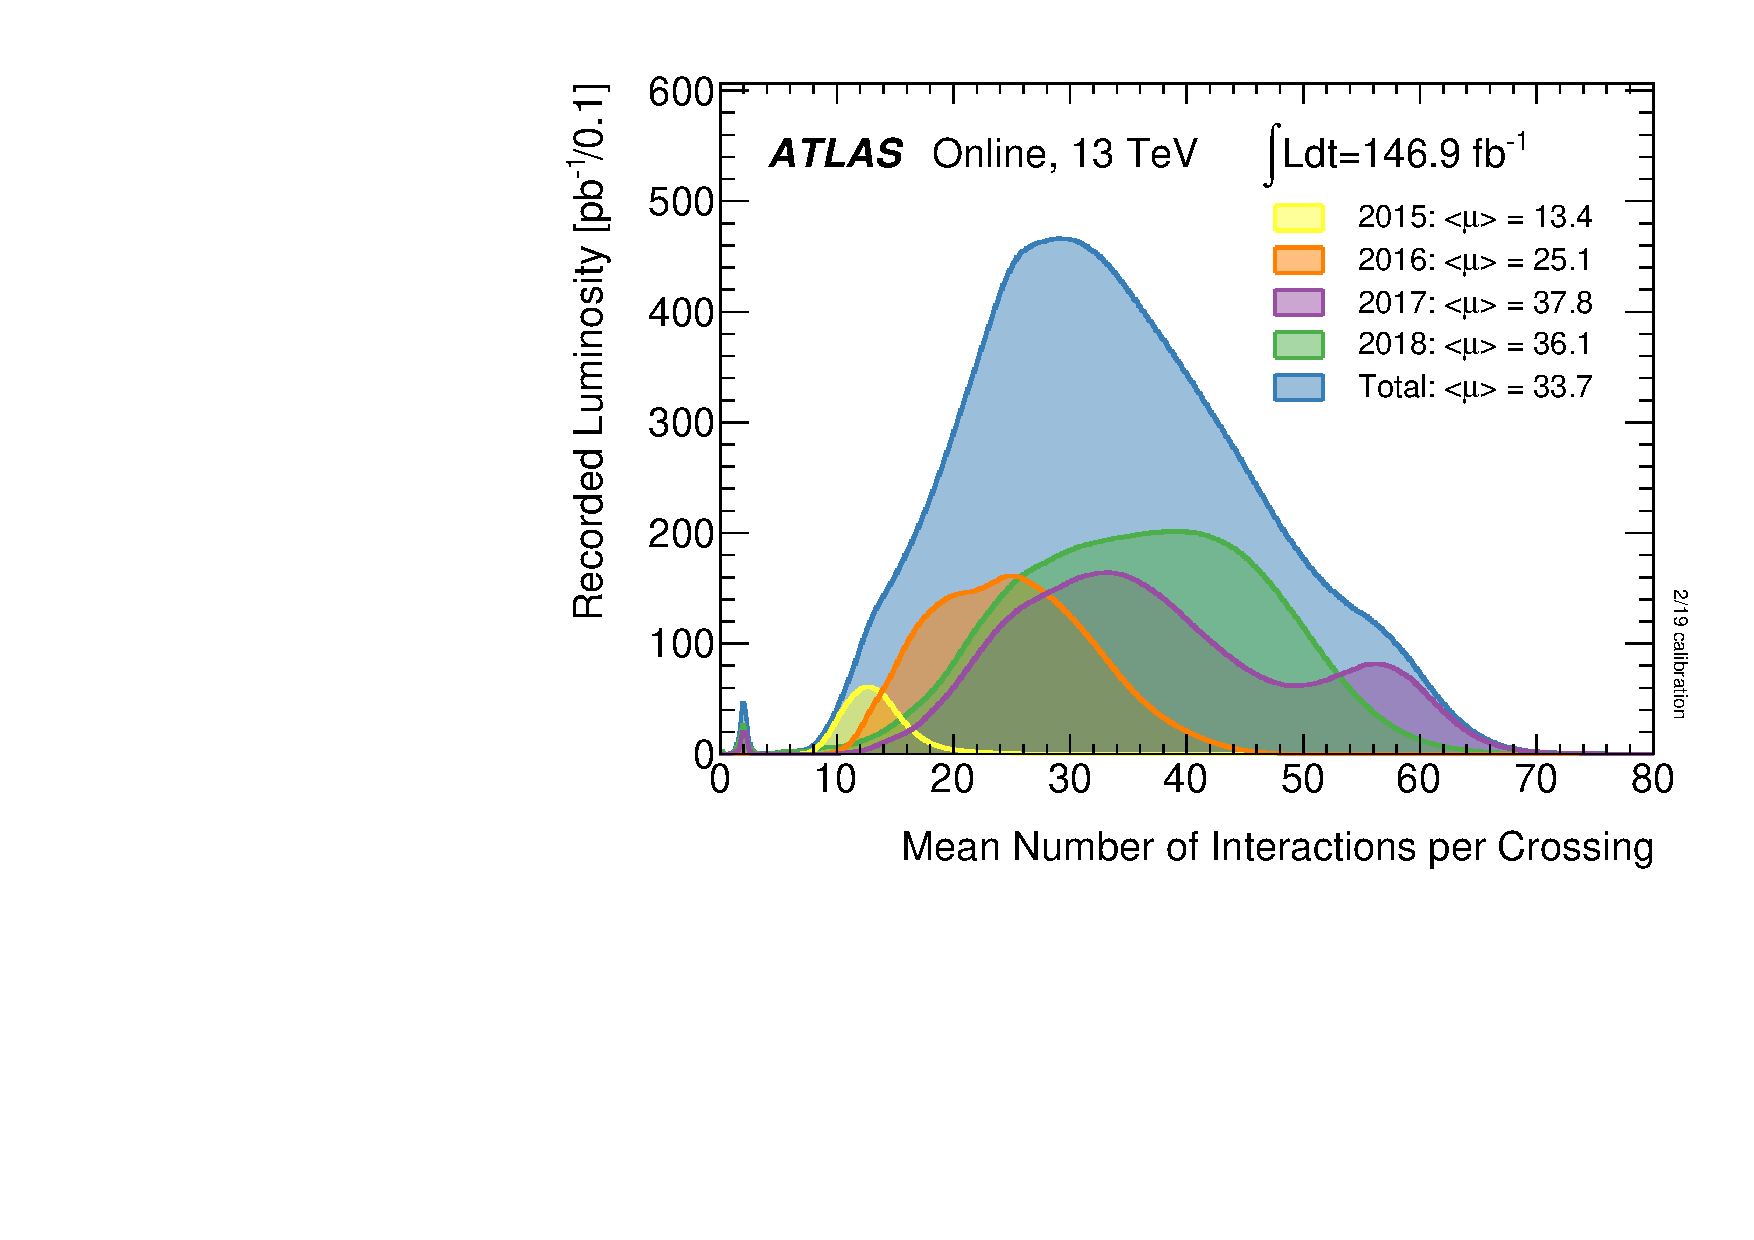
\includegraphics[width=0.5\textwidth]{mu_2015_2018}
        \caption[]{Pile up profiles for run 2 data taking periods \citep{pileup}.}
    \label{fig:pileup}    
\end{figure}

\subsection{The ATLAS detector}
The \ac{atlas} (A Toroidal LHC Apparatus) experiment is a particle detector with an onion-like structure, as shown in figure \ref{fig:atlas_detector}.
\begin{figure}
    \centering
    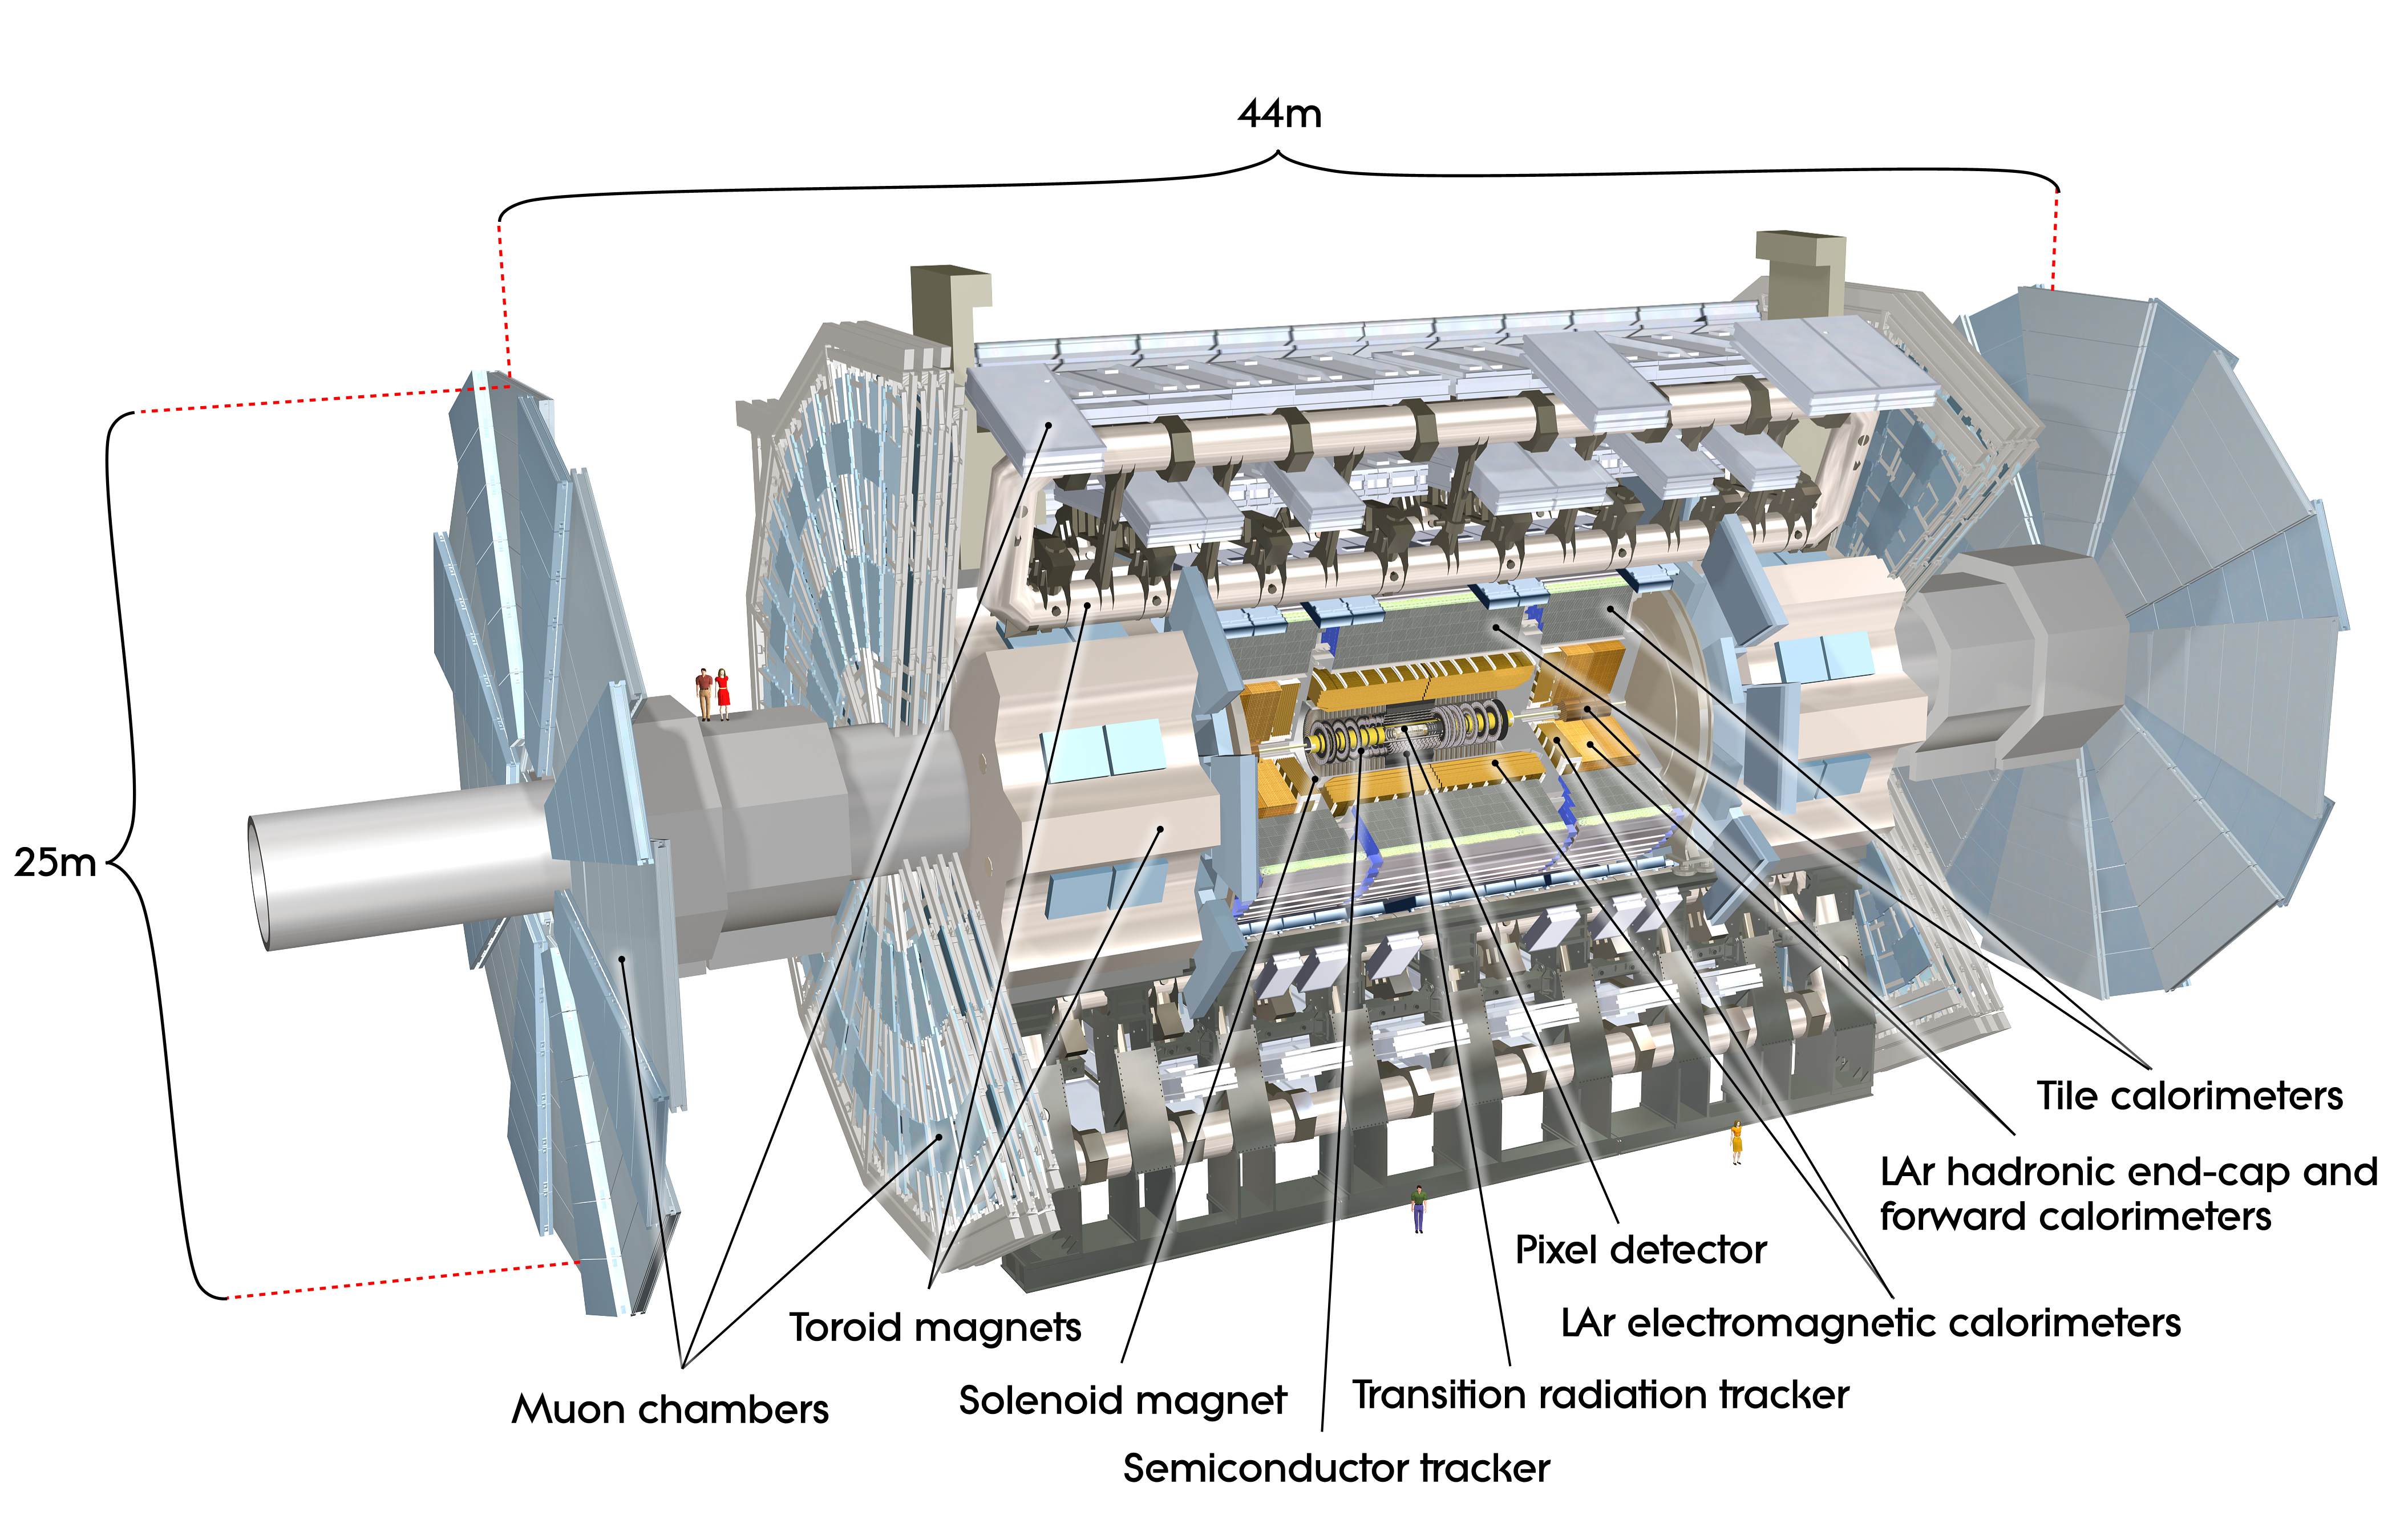
\includegraphics[width=1\textwidth]{atlas_detector}
        \caption[]{The \ac{atlas} experiment at the \ac{lhc} with its subdetectors. Adopted from \citep{Pequenao:1095924}.}
    \label{fig:atlas_detector}    
\end{figure}
Its purpose is to measure the trajectory, momentum, and energy of particles originating from proton-proton collisions, depending on the particular kind of interaction of the collision products with matter. The various subdetectors are explained below from the inside out.

\subsubsection*{Coordinate System}
The coordinate system of \ac{atlas} is right-handed and originates at the interaction point at the center of the detector. The z-axis points along the beam line, the x-axis to the center of the lhc and the y-axis away from earth. Thus quantities transversal to the z-axis are Lorentz-invariant. Inside the detector cylindrical coordinates $r,\phi$ are used with $\phi$ the azimuthal angle about the z-axis and the polar angle $\Theta$ of a particle measured in form of the pseudorapidity $\eta=-\ln(\Theta/2)$. This quantity is defined as an approximation for the Lorentz invariant rapidity and holds for highly relativistic particles. With these a useful quantity to describe angular distances in the detector is
\begin{equation}
    \Delta R = \sqrt{(\Delta\phi)^2+(\Delta eta)^2}.
\end{equation}

\subsection{Inner detector}
The inner detector, shown schematically in figure \ref{fig:inner_tracker}, is designed to track charged particles and figure out their momentum and provide information on the particle type. 
\begin{figure}
    \centering
    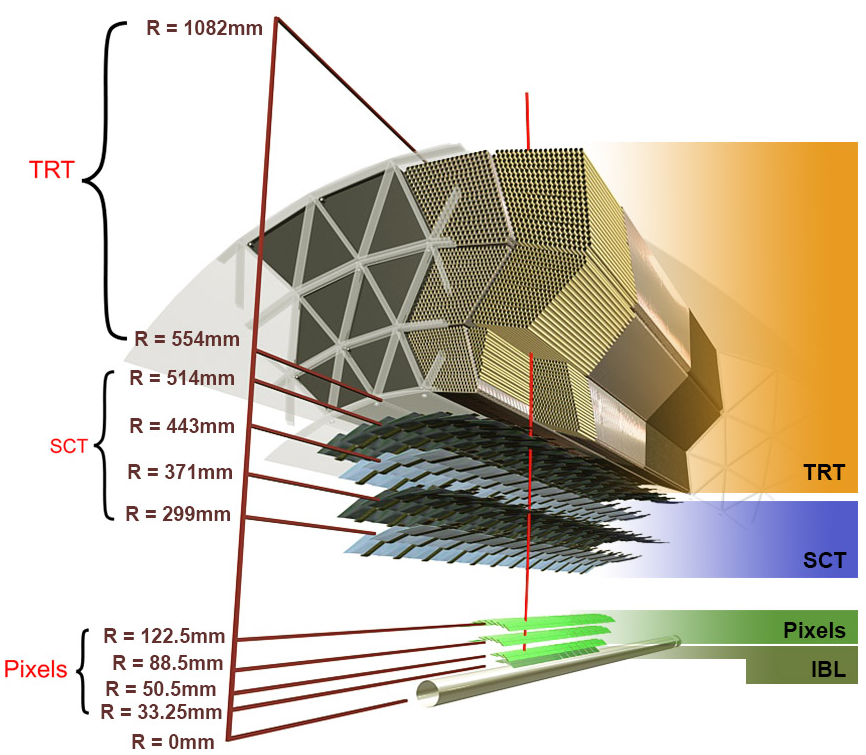
\includegraphics[width=0.65\textwidth]{inner_tracker}
        \caption[]{The inner detector schematically with the subdetectors described in the full text. Adopted from \citep{Potamianos:2016ptf}.}
    \label{fig:inner_tracker}    
\end{figure}
It is surrounded by a solenoid magnet whose field lines point in the direction the beam so that charged particles are bent in the transverse plane of the detector due to the Lorentz force. The bending direction reveals the charge whereas the curvature depends on the momentum.

The \ac{ibl}, pixel detector, and \ac{sct} all consist of silicon detectors of various sizes. When passing through silicon, charged particles ionize electrons that travel in an electric field to an electrode and provide positional information. The \ac{ibl} plays a crucial role in b-tagging as will become clear in section \red{add ref}.

After aforementioned semiconductor trackers the \ac{trt} surrounds them and is based on transition radiation and can also provide particle ID's. It consists of several layers of tubes perpendicular to the beamline, filled with a gas mixture, and a conducting wire in their center, which is under voltage and attracts negative charges. The tubes are embedded in polypropylene. Transition radiation is emitted when a charged particle passes through media with different permittivities at the boundary of the materials. The intensity of this radiation depends on the velocity, so that for particles of the same energy more photons are released for the lighter particle, so that for example electrons can be distinguished from pions.

